\pdfoutput=1

\documentclass[a4paper,openright,twoside,12pt]{book}
\setcounter{secnumdepth}{4}
\setcounter{tocdepth}{4}
\usepackage[left=4cm,top=3cm,right=3cm,bottom=4cm]{geometry}
\usepackage{amsmath,amssymb}
\usepackage{bm}
\usepackage{color}
\usepackage[latin1]{inputenc}
\usepackage[english]{babel}
\usepackage[T1]{fontenc}
\usepackage{t1enc}
\usepackage[pdftex]{graphicx}  % pdftex grafik
\usepackage{latexsym}
\usepackage{mathrsfs}
\usepackage{braket}
\usepackage{multicol}
\usepackage{dsfont}
\usepackage{fancyhdr}
\usepackage{float}
\usepackage{amsfonts}
\usepackage{amsmath}

\numberwithin{equation}{section}

\newcommand*{\Lastname}{Backes}
\newcommand*{\Firstname}{Steffen}
\newcommand*{\Supervisor}{Steffen Backes}

\newcommand*{\Typ}{Bachelor in Physics}
\newcommand*{\Title}{Density functional theory and dynamical mean-field theory: A way to model strongly correlated systems}
\newcommand*{\Subtitle}{~}
\date{}

\usepackage[
 pdfstartpage = {1},
colorlinks=false,
bookmarks=true,
bookmarksopen=true,
bookmarksnumbered=true,
pdftitle={\Title},
pdfauthor={\Firstname\ \Lastname},
pdfsubject={},
pdfkeywords={}
]{hyperref}
\hypersetup{
%    colorlinks=false,
   citecolor=red,
   linkcolor=red,
   urlcolor=blue,
citebordercolor = {1 0 1},
filebordercolor = {0 .5 .5},
linkbordercolor = {0 1 1},
menubordercolor = {1 1 0},
linktocpage = false,			
pdfhighlight = /I,			
pdfpagelayout = OneColumn,		
hypertexnames=false			
}
 			

\usepackage{fancyhdr}				
\pagestyle{fancy}				
\fancyhf{}					
\fancyhead[EL]{\thepage}		
\fancyhead[ER]{\leftmark}		
\fancyhead[OL]{\rightmark}		
\fancyhead[OR]{\thepage}		
\renewcommand{\chaptermark}[1]
{ \markboth{ \thechapter. \ #1}{}}
\renewcommand{\sectionmark}[1]{ \markright{\thesection{} #1} }

 \renewcommand{\topfraction}{0.75} 
 \renewcommand{\bottomfraction}{0.75}
 \setlength{\headheight}{16pt}
 

\begin{document}
\pagestyle{empty}
%
\begin{center}
\begin{minipage}{0.45\textwidth}

\includegraphics[width=1\textwidth]{ipp.jpg}
\end{minipage}
\hfill
\begin{minipage}{0.2\textwidth}

\includegraphics[width=1\textwidth]{polytechnique.png}
\end{minipage}\\
\vspace{1.5cm}
\Huge \textbf{ \Title } \\ 
\vspace{1.5cm}
\large 
\textit{A thesis submitted for the degree of\\
{\Typ}}\\
%
\vspace{0.5cm}
\large \textit{by}
\vspace{0.5cm}\\
\Large  \Firstname\ \Lastname
\vspace{0.5cm}\\
\large 
\textit{at the}
\vspace{0.5cm}\\
%
Centre de Physique Th\'eorique (CPHT) \\
Ecole Polytechnique \\
91128 Palaiseau cedex\\ 
France
%
\vspace{0.5cm}\\
\textit{under the supervision of}
\vspace{0.5cm}\\
%
\Large \Supervisor
\end{center}
\clearpage

\thispagestyle{empty}
\clearpage

\tableofcontents
\cleardoublepage

\pagestyle{fancy}

%%%%%%%%%%%%%%%%%%%%%%%%%%%%%%%%%%%%%

\chapter{Introduction}
\section{Introduction into correlated electron materials}
The concept of electronic correlations is one of the hardest, yet most interesting 
aspects in the field of theoretical as well as experimental solid state physics. 
This thesis will investigate the realisations of strong electronic correlations due
the Coulomb repulsion between electrons in different materials and theoretical concepts
of describing and investigating their effects on physical properties. 

In this chapter we will give a short overview over the main aspects of this thesis.
We will first introduce the very general problem of how an ensemble of electrons 
in a solid interacts and what problems arise when we want to investigate the system
from the viewpoint of a theoretical physicist.

After that, we will review a special type of materials, namely a class of 
superconductors in which electronic correlations are important to consider for a correct physical
description and interpretation of their properties. 

\chapter{Methods}
\section{The Hubbard model}
In order to find a way of appropriately treating electronic correlations we should also consider alternative ways
of treating the Coulomb repulsion. Since the Coulomb interaction is a long-range interaction due to the potential
falling off as $\sim \frac{1}{r}$, the problem is notoriously difficult since we need to take the contribution
of many particles into account. However, in real systems the range of the interaction is effectively reduced due
to screening effects of the electronic charge. Consider electrons moving in a positive background potential given
by the atomic lattice. Focussing on a specific electron, one will observe a region of reduced electronic density 
in the vicinity of said electron due to the Coulomb repulsion, that creates an effective positively charged
cloud that will move around with the electron. From large distances, the resulting potential seen
by other electrons will thus be reduced by the positive cloud compared to the bare electron.
Therefore, the effective potential will fall off much faster than the bare Coulomb repulsion,
making it an effective short-range interaction. This is why approximative
models like the Hubbard model~\cite{Gutzwiller1963,Hubbard1963,Kanamori1963}, which assume the Coulomb repulsion
to be completely local, can be quite appropriate to describe correlated lattice systems.

The most simple variant is the one-band fermionic Hubbard model, given by the Hamiltonian
\begin{align}
H 
&= \sum_{\langle i,j\rangle,\sigma} t_{ij} c^{\dagger}_{i\sigma}c_{j\sigma}
  + U \sum_{i}  n_{i\uparrow} n_{i\downarrow},
\end{align}
with the hopping amplitudes $t_{ij}$ between neighbouring sites $i,j$. The Coulomb interaction is 
represented by a local on-site interaction $U$, that has to be paid if two electrons of opposite spin occupy 
the same site. Fig.~\ref{dmft:fig:hubbard_model_lattice} shows an example of the two-dimensional Hubbard model.
It can encompass basically all types of lattice systems by appropriately choosing the hopping integrals $t_{ij}$.
%
\begin{figure}[t]
\begin{center}
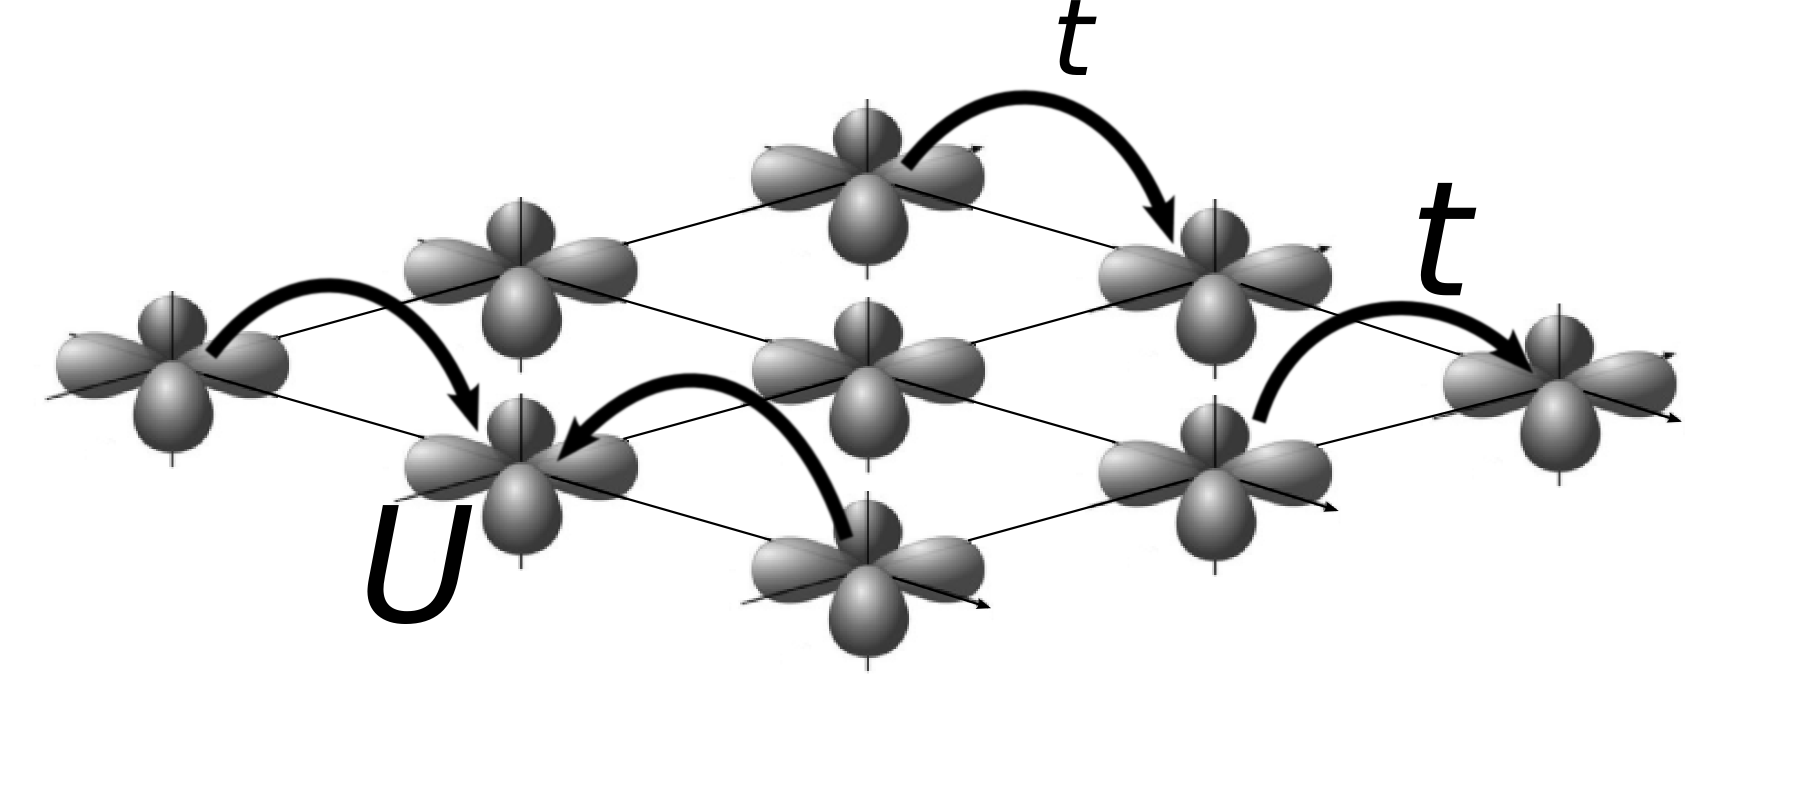
\includegraphics[width=0.7\textwidth]{hubbard_lattice.png}
\end{center}
\caption{Illustration of the one-band Hubbard model in two dimensions. The model consists of a lattice of atomic sites
occupied by electrons that can hop between neighbouring sites with the hopping amplitude $t$.
Double occupation of an atomic site with two electrons of the opposite spin incurs an energy penalty
of $U$ to mimic the screened short-range Coulomb interaction.
.}
\label{dmft:fig:hubbard_model_lattice}
\end{figure}
%
Even though this model appears to be very simple, it is not only impossible to be solved analytically in more than one 
dimensions~\cite{Lieb1968}, but also includes the main effects of the competition between the kinetic energy
and Coulomb interaction.
Considering for example the limit $U/t\rightarrow 0$, the Hamiltonian  corresponds to that of free particles 
with a dispersion corresponding to the Fourier transform of $t_{ij}$ For the linear chain
we already had as an example $\epsilon(k)=-2t\cos(ka)$ and, since the Hamiltonian separates into a sum of single-particle
terms, all expectation values can be calculated independently. Thus, all correlation functions factorize, e.g.
\begin{align}
\langle n_{i\uparrow} n_{i\downarrow} \rangle 
&= \langle n_{i\uparrow} \rangle \langle n_{i\downarrow} \rangle.
\end{align}
%
Considering the other limit of $U/t\rightarrow \infty$, the Hamiltonian becomes just the sum of the double occupations
times $U$. At half filling the ground state which minimizes the energy thus corresponds to each electron being localized
on an atomic site with zero probability on all other sites. As a result, the system is now in an insulating state
due to the electronic correlations and the correlation functions no longer factorize
\begin{align}
\underbrace{\langle n_{i\uparrow} n_{i\downarrow} \rangle}_{=0} 
&\neq \underbrace{\langle n_{i\uparrow} \rangle}_{=0.5} \underbrace{\langle n_{i\downarrow} \rangle}_{=0.5}.
\end{align}
Thus, even though the Hubbard model is quite simple, it can show the non-trivial effect of a {\mit}
as $U/t$ is increased. Approximations like Hartree-Fock theories that are based on the separation of correlation
functions are, therefore, also insufficient to correctly describe the physics in the Hubbard model for strong
interactions. 

\chapter{Result \& Interpretation}
\section{First experiment}

\section{Second experiment}

\chapter{Conclusion \& Outlook}


%
%

\renewcommand\bibname{References}
\bibliographystyle{unsrt}
\bibliography{references}
\addcontentsline{toc}{chapter}{References}

\end{document}
